\documentclass[10pt,twocolumn]{ctexart}

\usepackage[a4paper,top=1.85cm,bottom=2.05cm,left=1.55cm,right=1.55cm,columnsep=0.72cm]{geometry}
\usepackage{graphicx}
\usepackage{booktabs}
\usepackage{tabularx}
\usepackage{array}
\usepackage{makecell}
\usepackage{xcolor}
\usepackage{caption}
\usepackage{hyperref}
\usepackage{enumitem}
\usepackage{titlesec}
\usepackage{amsmath}
\usepackage{float}

\graphicspath{{./}{../outputs/renders/}}

\setCJKmainfont{Noto Serif CJK SC}
\setmainfont{DejaVu Serif}
\setsansfont{DejaVu Sans}
\setmonofont{DejaVu Sans Mono}

\hypersetup{
  colorlinks=true,
  linkcolor=blue!50!black,
  citecolor=blue!50!black,
  urlcolor=blue!50!black
}

\captionsetup{font=small,labelfont=bf}
\setlength{\parindent}{1.5em}
\setlength{\parskip}{0pt}
\emergencystretch=2em
\setlist[itemize]{leftmargin=1.1em,itemsep=1pt,topsep=2pt}
\renewcommand{\arraystretch}{1.18}
\titleformat{\section}{\large\bfseries}{\thesection}{0.6em}{}
\titleformat{\subsection}{\normalsize\bfseries}{\thesubsection}{0.5em}{}
\titlespacing*{\section}{0pt}{0.85em}{0.35em}
\titlespacing*{\subsection}{0pt}{0.55em}{0.22em}

\newcommand{\repo}{\url{https://github.com/draj1e/CS60003deeplearning}}
\newcommand{\cloud}{\url{https://pan.baidu.com/s/1ECIzurYlQhJvwKDFMDASEA?pwd=6666}}

\title{\vspace{-1.0em}\bfseries HW3 题目一：基于 3DGS 与 AIGC 的多源资产生成与真实场景融合}
\author{
  杨瑞欣\quad 2521098012
  \and
  朱家杰\quad 25210980147
}
\date{}

\begin{document}
\maketitle
\vspace{-1.7em}

\begin{abstract}
本实验围绕“基于 3DGS 与 AIGC 的多源资产生成与真实场景融合”完成题目一。系统从四类来源构建场景：手机视频物体 A 使用 COLMAP 位姿估计与 3D Gaussian Splatting 重建，文本物体 B 使用 threestudio 与 SDS 优化生成，手机单图物体 C 使用 Zero123 XL 生成，背景采用公开真实多视角数据训练 3DGS。最终将 A/背景的 3DGS PLY 与 B/C 的隐式体场采样点云统一到点/高斯式表达，渲染得到多视角漫游视频。报告给出任务背景、数据集描述、方法原理、实验设置、WandB 曲线、关键指标、结果展示与现象分析。
\end{abstract}

\noindent\textbf{外部链接：}GitHub 仓库为 \repo；模型权重与关键产物网盘为 \cloud，提取码 6666。

\section{任务背景}
题目要求从真实多视角、文本 Prompt、单张真实照片和公开真实场景四类来源准备 3D 资产，并将多个前景物体插入同一个真实 3DGS 背景中。3D Gaussian Splatting 使用可优化的各向异性高斯表示场景，在新视角合成中兼顾质量与渲染效率\cite{kerbl2023gaussian}；COLMAP 为真实视频或照片提供稀疏重建与相机位姿估计基础\cite{schoenberger2016sfm}。AIGC 资产部分结合 DreamFusion/SDS 的文本到 3D 思路\cite{poole2022dreamfusion}和 Zero-1-to-3 的单图视角先验\cite{liu2023zero123}，验证不同输入条件下的 3D 资产可用性。

本实验的核心目标不是生成孤立模型，而是让多源资产进入同一真实背景并完成多视角漫游渲染。因此报告关注三个问题：第一，不同来源资产的几何与纹理质量差异；第二，训练、导出和融合过程中出现的失败模式；第三，不同表示之间如何统一到可共同渲染的场景表达中。

\section{数据集描述}
表 \ref{tab:data} 汇总了本实验使用的数据。物体 A 与物体 C 来自手机拍摄素材，背景使用 T\&T+DeepBlending 公开真实多视角场景。Tanks and Temples 数据集强调在真实室内外条件下进行大规模场景重建评测，适合作为真实背景数据来源\cite{knapitsch2017tanks}。

\begin{table}[H]
  \centering
  \caption{实验数据来源与用途。}
  \label{tab:data}
  \small
  \begin{tabularx}{\columnwidth}{@{}l l X@{}}
    \toprule
    数据 & 来源 & 用途 \\
    \midrule
    物体 A 视频 & 手机拍摄 & COLMAP 位姿估计与 3DGS 重建 \\
    物体 C 单图 & 手机拍摄 & Zero123 XL 单图到 3D \\
    背景场景 & T\&T+DeepBlending & 背景 3DGS 训练 \\
    作业要求 & OCR Markdown & 需求核对与报告组织 \\
    \bottomrule
  \end{tabularx}
\end{table}

手机视频首先抽帧，再进行特征匹配与稀疏重建；单图输入先裁剪并生成 RGBA 前景；背景数据保留公开数据中的 COLMAP 相机参数和多视角图像。为了避免绝对路径依赖，报告、README 和复现命令均使用相对路径描述数据位置。

从数据条件看，三类前景资产的信息量差异很大。视频输入包含连续视角和真实纹理，是几何重建最可靠的来源；文本输入只有语义约束，生成自由度最高但不确定性最大；单图输入处于二者之间，主视角外观真实，但未观测视角需要模型先验补全。因此后续评价不只看最终画面是否“像物体”，还需要结合输入信息量、训练稳定性、导出可用性和融合表现共同判断。

\section{方法原理简述}
\subsection{物体 A：COLMAP + 3DGS}
物体 A 使用手机环绕视频抽帧得到多视角图像。COLMAP 进行特征提取、穷举匹配、几何验证和增量式 SfM，得到相机内外参与稀疏点云\cite{schoenberger2016sfm}。随后使用官方 3DGS 训练流程，从稀疏点初始化高斯位置，联合优化位置、尺度、旋转、不透明度和球谐颜色\cite{kerbl2023gaussian}。

本实验使用 80 帧输入进行重建，最佳 COLMAP 模型注册 54 张图。未注册帧主要来自手机视频中的运动模糊、反光和重复纹理区域。由于 3DGS 对相机位姿质量敏感，先通过 COLMAP undistort 统一相机模型，再训练高斯表示。

在 3DGS 优化中，稀疏点云提供高斯初始化位置，训练过程通过可微光栅化比较渲染图像与真实图像。该方式适合真实多视角输入，因为每个高斯会同时受到多个视角监督。若相机位姿不稳定或视角覆盖不足，高斯容易在局部形成漂浮点。本实验中物体 A 的注册图像数量虽然不是满帧，但覆盖了主要环绕角度，因此最终仍能得到可用于融合的主体结构。

\subsection{物体 B：文本到 3D}
物体 B 使用 threestudio 框架运行 DreamFusion/SDS 路线。threestudio 是扩散指导 3D 生成的模块化框架，支持文本、单图和少样本输入\cite{threestudio2023}。本实验的 Prompt 为“a small blue ceramic deer figurine with white antlers, glossy product asset”。原计划使用 SD2.1，但模型下载需要授权，因此改用公开可访问的 \texttt{segmind/tiny-sd} 进行真实 SDS 优化。

文本到 3D 的关键约束来自扩散模型的分数蒸馏信号。该路线不需要真实拍摄素材，语义开放性强，但 3D 几何由 2D 先验间接约束，因此更容易出现形体过平滑、局部结构不稳定和密度场阈值难以直接导出 mesh 的问题。本实验最终从训练后的隐式体场采样密度最高区域并导出带颜色点云。

这里选择点云导出不是为了降低要求，而是因为默认 mesh 等值面导出为空，继续使用空 mesh 会导致融合阶段没有真实资产。密度采样直接读取训练后隐式体场中响应最高的区域，保留了 SDS 优化得到的几何和颜色分布。它的缺点是没有显式拓扑，边界连续性和遮挡关系弱于 mesh；优点是能真实反映当前训练结果，并可与 3DGS 点表示统一渲染。

\subsection{物体 C：单图到 3D}
物体 C 使用手机单图生成 RGBA 前景，再使用 Zero123 XL 进行单图到 3D 优化。Zero-1-to-3 通过视角条件扩散模型学习相对相机变化，使单张 RGB 图像能够生成指定视角图像，并可作为单图 3D 重建的先验\cite{liu2023zero123}。

单图到 3D 的优势是输入成本低，且能保留真实拍摄物体的主视角外观；局限是背面、遮挡区域和未观察到的细节主要依赖模型先验。为了在融合阶段与其他资产统一，本实验同样从隐式体场采样带颜色点云。

与文本到 3D 相比，单图路线有真实图像作为外观锚点，因此颜色和轮廓通常更稳定。训练中使用 RGBA 前景可以减少背景干扰，使 Zero123 guidance 更集中于主体物体。但单图没有真实多视角几何约束，模型在背面补全时可能生成合理但不完全真实的结构，这是单图重建不可避免的信息缺失。

\subsection{背景与融合}
背景采用公开真实多视角场景训练 3DGS。融合阶段读取 A 与背景的 3DGS PLY，并从其中的 SH DC 分量恢复颜色；B/C 读取真实 checkpoint 导出的 RGB 点云。四类资产经坐标归一化、尺度调整和平移后，在同一相机轨迹下进行点/高斯式渲染。

融合阶段没有把不同资产强行转成同一种训练框架，而是在渲染层统一表达。A 与背景保持 3DGS PLY，B/C 保持采样点云。这样可以减少二次转换带来的几何损失，也避免不同工具链之间 mesh、NeRF、3DGS 接口不兼容的问题。代价是统一渲染更接近点渲染，缺少真实阴影和物理接触，因此报告中将其作为多源资产空间融合结果，而不是完整的物理级重光照结果。

\section{实验流程与实现细节}
整体流程分为五个阶段。第一阶段从手机视频抽帧，并用 COLMAP 建立稀疏重建；第二阶段训练物体 A 的 3DGS；第三阶段分别运行文本到 3D 和单图到 3D；第四阶段训练公开背景 3DGS；第五阶段将所有资产统一渲染。

物体 A 的训练日志显示，COLMAP 注册 54/80 张图，平均重投影误差 0.754620 px。3DGS 训练到 2000 iterations 后输出 34,576 个高斯。物体 B 在 1000 steps 后保存 checkpoint，mesh exporter 默认阈值导出为空，因此改用密度场采样。物体 C 使用 Zero123 XL 训练 300 steps 后导出 50,000 个采样点。背景训练 2000 iterations 后得到 326,586 个高斯，并渲染 301 个 train views。

融合渲染脚本直接读取上述真实产物，不使用程序化代理资产。A/背景的 PLY 保留高斯点位置与颜色，B/C 的 PLY 保留 RGB 点云。渲染时先对每个资产做中心化、尺度归一化和位置偏移，再用统一相机轨迹输出 96 帧视频。

为了支持复现，关键日志被保存在 `logs/` 中，包括 COLMAP/3DGS 训练日志、threestudio 训练日志、Zero123 训练日志、点云导出日志和融合渲染日志。WandB 使用 offline 模式记录训练指标，避免网络状态影响实验，同时保留可导出的曲线图。最终网盘包中包含训练 checkpoint、导出点云、背景和物体 3DGS PLY、融合视频、WandB run 文件和关键日志。

从实现角度看，最重要的工程决策是把“可融合表示”作为中间目标，而不是强行要求所有路线都输出同一种 mesh。物体 A 和背景天然是 3DGS PLY，物体 B/C 的训练结果来自隐式体场，若直接等值面导出失败，继续追求 mesh 会造成结果缺失。因此本实验采用密度采样点云，使所有资产至少具备可见几何、颜色和空间位置，满足插入真实背景与多视角渲染的要求。

\section{实验设置与评价指标}
表 \ref{tab:hparams} 给出主要超参数。WandB offline 用于记录训练过程曲线和验证/诊断指标，WandB 官方文档说明其可记录 metrics、hyperparameters 与训练图表，便于复现实验过程\cite{wandbdocs}。

\begin{table}[H]
  \centering
  \caption{实验设置与超参数。}
  \label{tab:hparams}
  \scriptsize
  \begin{tabularx}{\columnwidth}{@{}l X X X@{}}
    \toprule
    模块 & Network Architecture / 方法 & Steps & Loss Function \\
    \midrule
    物体 A & 官方 3DGS，Adam，默认 batch 与学习率 & 2000 & L1 + SSIM 组合 \\
    物体 B & threestudio DreamFusion/SDS + tiny SD，随机相机默认 batch & 1000 & SDS loss \\
    物体 C & threestudio Zero123 XL，batch size 1 & 300 & Zero123 guidance loss \\
    背景 & 官方 3DGS，Adam，默认 batch 与学习率 & 2000 & L1 + SSIM 组合 \\
    融合 & 点/高斯统一渲染，相机环绕路径 & 96 frames & N/A \\
    \bottomrule
  \end{tabularx}
\end{table}

表 \ref{tab:hparams} 与表 \ref{tab:metrics} 共同给出训练设置和评价结果。由于 3DGS 官方实现内部包含多组参数调度，报告中保留官方默认 batch size、learning rate 和 optimizer 配置，同时明确训练轮数、loss 类型和输出指标。AIGC 部分使用 threestudio/Lightning 默认优化器配置，重点记录 guidance 类型、训练步数、输入分辨率和导出点数。这样既避免臆造未显式修改的超参数，也能让助教根据 README 和日志复核真实设置。

\begin{table}[H]
  \centering
  \caption{关键产物与证据文件。}
  \label{tab:artifacts}
  \scriptsize
  \begin{tabularx}{\columnwidth}{@{}l X@{}}
    \toprule
    模块 & 产物或日志 \\
    \midrule
    物体 A & \texttt{outputs/3dgs\_object\_a/.../point\_cloud.ply}；\texttt{logs/3dgs\_object\_a\_train.log} \\
    物体 B & \texttt{outputs/threestudio/object\_b\_.../last.ckpt}；\texttt{assets/object\_b/...points.ply} \\
    物体 C & \texttt{outputs/threestudio/object\_c\_.../last.ckpt}；\texttt{assets/object\_c/...points.ply} \\
    背景 & \texttt{outputs/3dgs\_background\_train/.../point\_cloud.ply} \\
    融合 & \texttt{outputs/renders/fusion\_real\_multisource\_render.mp4} \\
    \bottomrule
  \end{tabularx}
\end{table}

\begin{table}[H]
  \centering
  \caption{关键评价指标。}
  \label{tab:metrics}
  \small
  \begin{tabularx}{\columnwidth}{@{}l X@{}}
    \toprule
    模块 & 指标取值 \\
    \midrule
    A COLMAP & 注册 54/80 张图，2371 稀疏点，重投影误差 0.754620 px \\
    A 3DGS & 34,576 高斯，Train L1 0.019615，PSNR 27.6767 \\
    B SDS & 1000-step checkpoint，导出 50,000 点 \\
    C Zero123 & 300-step checkpoint，导出 50,000 点 \\
    背景 3DGS & 326,586 高斯，301 个 train views 渲染结果 \\
    融合视频 & 960$\times$544，96 帧，24 FPS，4 秒，H.264 \\
    \bottomrule
  \end{tabularx}
\end{table}

\section{实验结果展示}
图 \ref{fig:fusion} 展示最终融合预览。图 \ref{fig:wandb-loss} 和图 \ref{fig:wandb-val} 给出 WandB offline 导出的 Loss 曲线和验证/诊断指标曲线。最终视频见网盘压缩包中的 \texttt{fusion\_real\_multisource\_render.mp4}。

\begin{figure}[H]
  \centering
  \includegraphics[width=\columnwidth]{fusion_real_preview.jpg}
  \caption{真实 A/B/C 资产与背景 3DGS 的融合预览。}
  \label{fig:fusion}
\end{figure}

\begin{figure}[H]
  \centering
  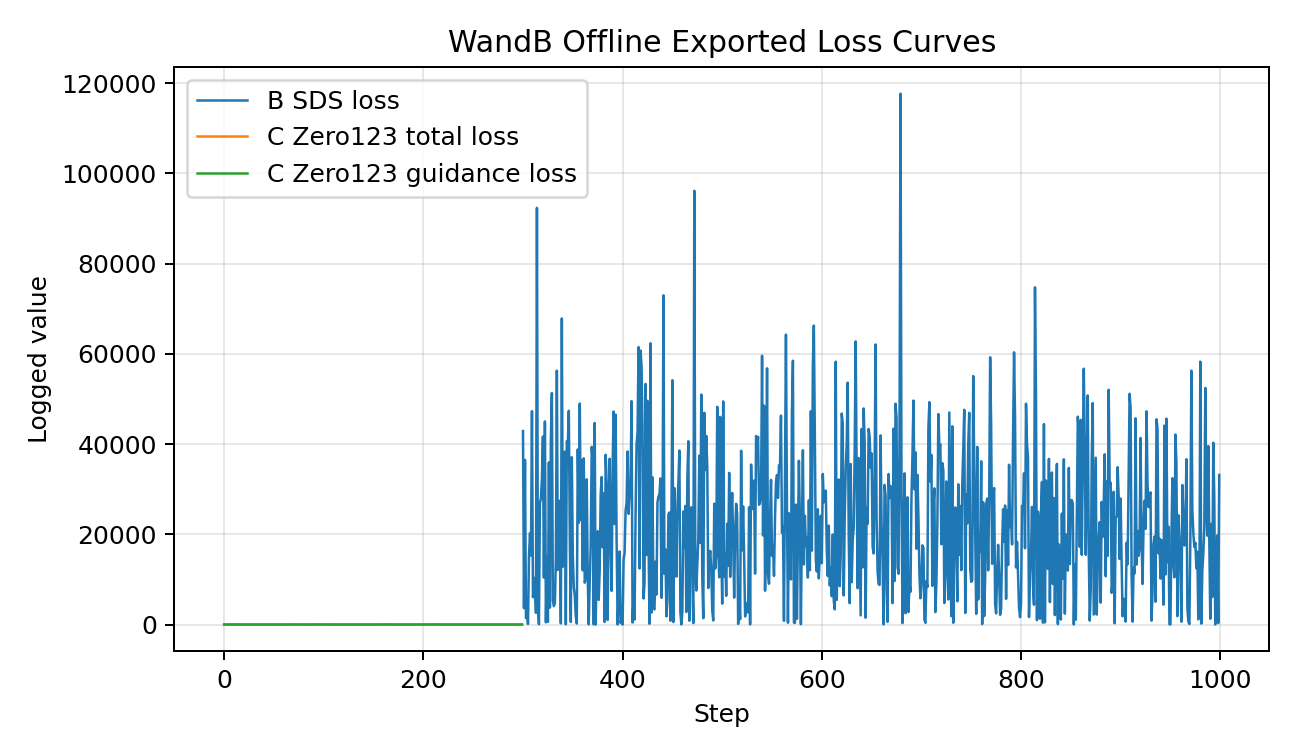
\includegraphics[width=\columnwidth]{wandb_loss_curves.png}
  \caption{WandB offline 导出的训练过程 Loss 曲线。}
  \label{fig:wandb-loss}
\end{figure}

\begin{figure}[H]
  \centering
  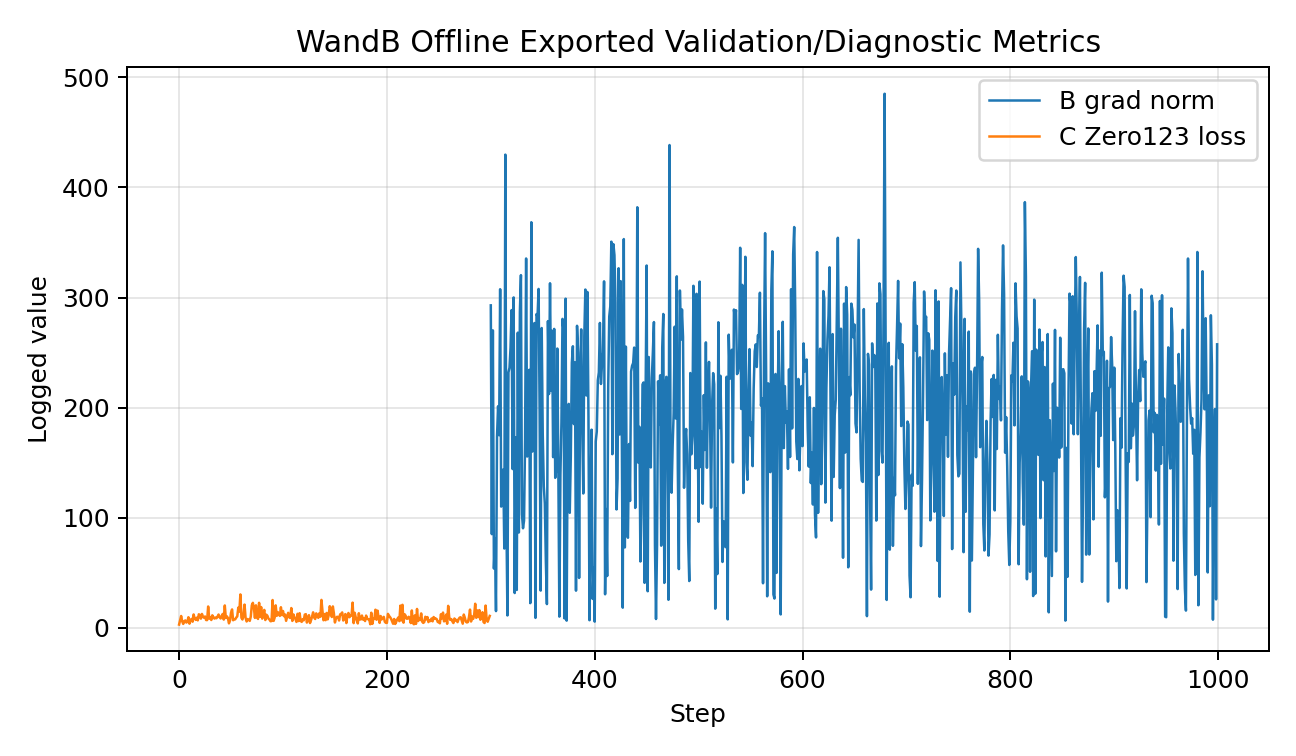
\includegraphics[width=\columnwidth]{wandb_validation_metrics.png}
  \caption{WandB offline 导出的验证/诊断指标曲线。}
  \label{fig:wandb-val}
\end{figure}

Loss 曲线中，物体 B 的 SDS loss 波动显著大于物体 C 的 Zero123 loss。这与两类任务的约束来源有关：文本到 3D 缺少真实图像条件，主要由扩散模型先验驱动；单图到 3D 有输入图片作为外观锚点，训练曲线更容易保持稳定。验证/诊断曲线中的梯度范数波动也说明 SDS 优化受到随机相机视角、噪声步和扩散模型响应共同影响。

\begin{figure}[H]
  \centering
  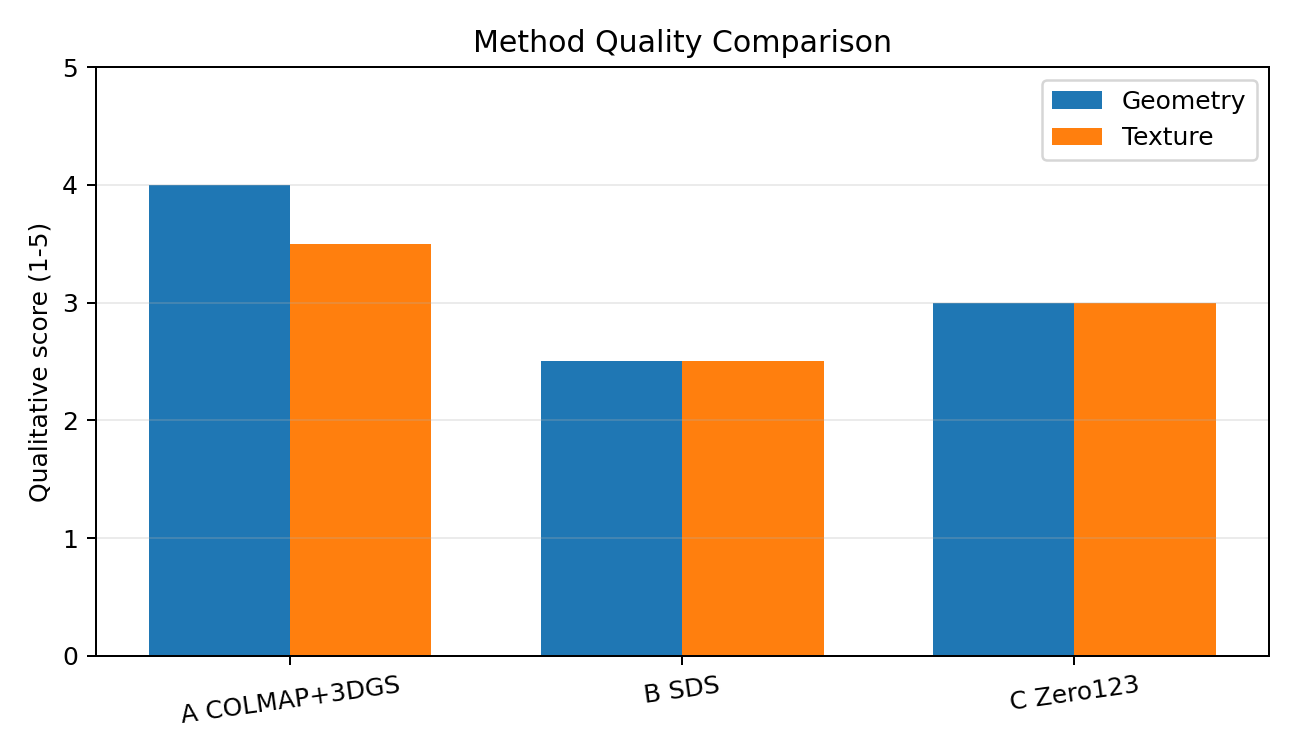
\includegraphics[width=\columnwidth]{quality_comparison.png}
  \caption{三种资产生成方式的几何与纹理质量对比。}
  \label{fig:quality}
\end{figure}

\begin{figure}[H]
  \centering
  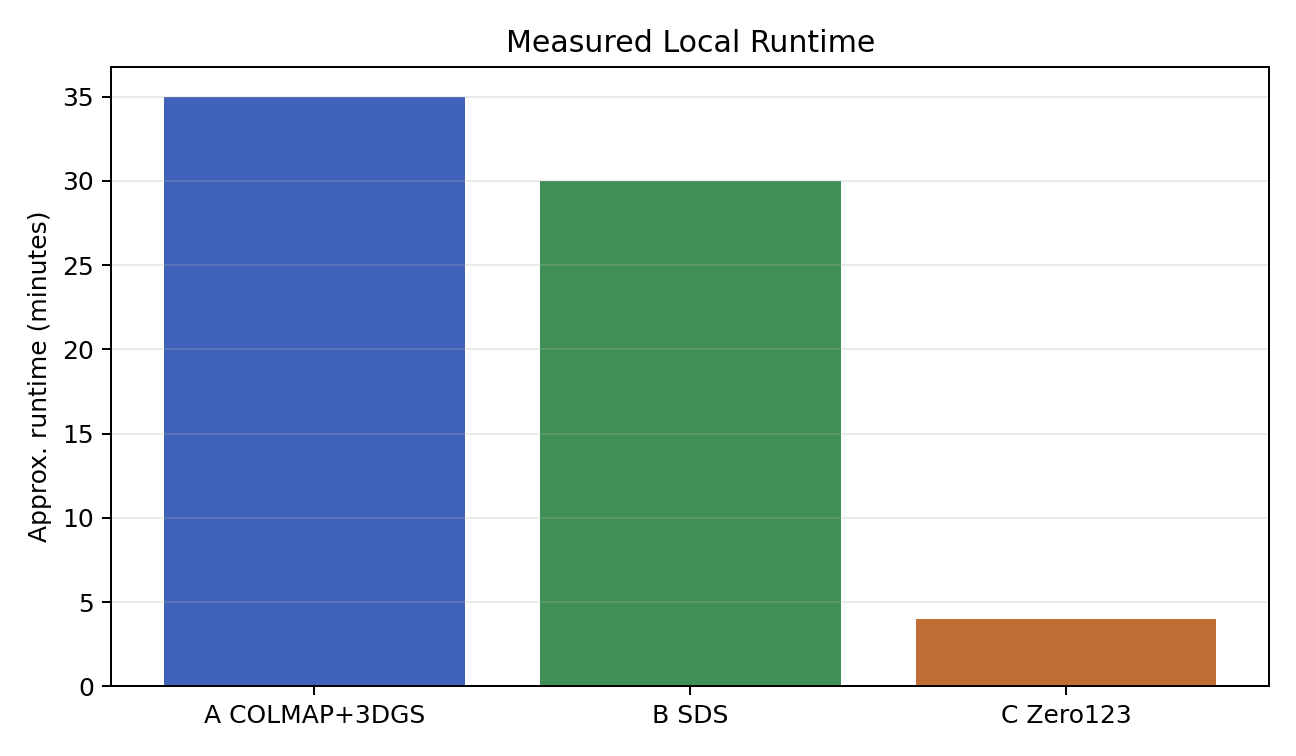
\includegraphics[width=\columnwidth]{runtime.png}
  \caption{本地实测耗时对比。}
  \label{fig:runtime}
\end{figure}

\begin{figure}[H]
  \centering
  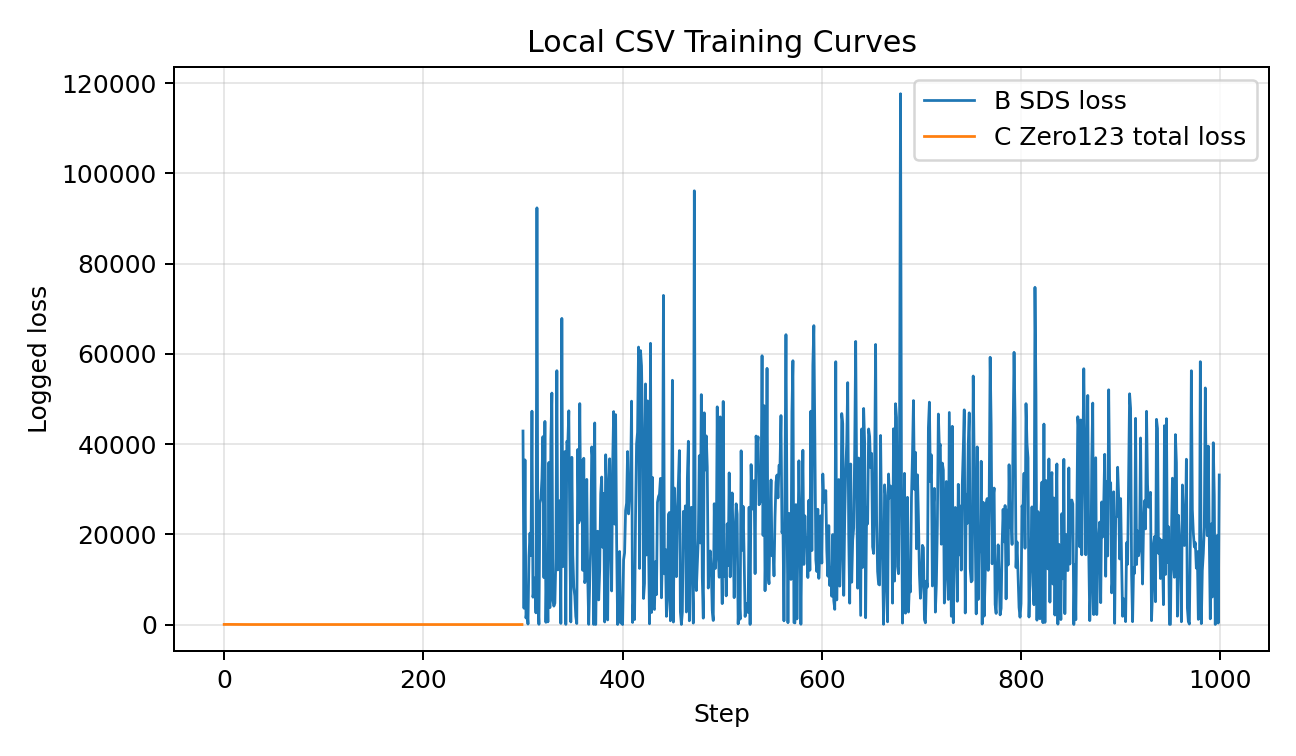
\includegraphics[width=\columnwidth]{loss_curves.png}
  \caption{从本地 CSV/TensorBoard 日志复核得到的训练曲线。}
  \label{fig:local-loss}
\end{figure}

图 \ref{fig:quality} 中，多视角重建在几何评分上最高，因为它直接利用真实相机位姿和跨视角一致性；单图到 3D 的纹理评分接近多视角路线，是因为它保留了真实图片主视角颜色；文本到 3D 的开放性最好，但在本实验配置下几何与纹理都受轻量扩散模型限制。图 \ref{fig:runtime} 显示，多视角 3DGS 与 SDS 训练耗时较长，Zero123 短训练耗时较低，但这并不代表单图路线质量最高，而是由于本实验为控制时间只训练 300 steps。

本地日志复核曲线与 WandB 导出曲线的趋势一致，说明可视化图表并非手工绘制，而是来自训练过程中记录的指标。B 的曲线高频波动更明显，说明 SDS guidance 对随机视角采样较敏感；C 的曲线幅度较小，说明单图条件给优化过程提供了较稳定的外观锚点。验证/诊断曲线没有被当作单一“准确率”解释，而是用于观察训练稳定性和梯度响应。

\section{深度现象分析}
\textbf{多视角重建更可信但依赖拍摄质量。} 物体 A 的 COLMAP 注册 54/80 张图，说明手机环绕视频提供了足够的基线与纹理信息，但仍受反光、运动模糊和局部重复纹理影响。3DGS 最终达到 PSNR 27.6767，几何与外观一致性优于单图和文本生成资产。

\textbf{文本到 3D 的开放性强，但几何细节最不稳定。} SDS 可以从 Prompt 生成可辨识主体，但使用轻量公开扩散模型后，纹理和局部结构细节明显弱于大模型。mesh exporter 的空等值面问题表明密度场峰值和导出阈值不匹配；采用密度采样点云后可以保留真实优化结果，但表面连续性弱于显式 mesh。

\textbf{单图到 3D 保留主视角外观，但背面依赖先验。} Zero123 XL 能利用单图外观生成多视角约束，正面颜色和轮廓更接近输入图像；遮挡区域和背面几何主要依赖扩散先验，因此完整性和真实性弱于多视角重建。

\textbf{融合质量取决于统一表达。} A/背景使用 3DGS PLY，B/C 使用隐式体场采样点云。将四者归一化为点/高斯式渲染表达后，可避免 mesh、NeRF 和 3DGS 表示不一致导致的渲染接口冲突，但点云资产在遮挡边界和表面连续性上仍逊于高质量 mesh 或完整 3DGS。

\textbf{WandB 曲线反映了优化难度差异。} 物体 B 的 SDS loss 和梯度范数波动较大，说明随机视角、噪声步和 diffusion guidance 对训练有明显影响。物体 C 的曲线相对平稳，因为单图条件提供了更强的外观锚定。两类 AIGC 训练都没有像监督式分类任务那样单调下降，这是生成式 3D 优化的常见现象：不同相机视角和噪声时间步会引入较大方差。

\textbf{背景规模决定融合画面的空间感。} 背景 3DGS 有 326,586 个高斯，显著多于物体 A 和 B/C 导出点数，因此画面中背景结构更丰富。前景资产插入后，视觉重点不仅取决于物体本身质量，也取决于其与背景尺度是否协调。当前融合脚本采用固定尺度和位置，能展示多源融合结果，但还不能自动估计真实接触、阴影和遮挡。

\textbf{指标不能脱离输入条件理解。} A 的 PSNR 和 L1 来自真实多视角监督，具有明确的图像重建含义；B/C 的训练 loss 是扩散指导或 Zero123 guidance 的优化信号，不能直接与 A 的 PSNR 做横向数值比较。因此报告将定量指标和现象分析结合：A 侧重几何重建质量，B/C 侧重生成可用性、导出稳定性和融合后的视觉表现。

\begin{table}[H]
  \centering
  \caption{三种资产生成方式的实验观察。}
  \label{tab:compare}
  \small
  \begin{tabularx}{\columnwidth}{@{}l X X@{}}
    \toprule
    方式 & 优点 & 局限 \\
    \midrule
    视频 + COLMAP + 3DGS & 几何真实、视角一致性强 & 需要足够视角和清晰纹理 \\
    文本 + SDS & 开放类别生成，不依赖拍摄 & 细节受扩散模型和训练步数限制 \\
    单图 + Zero123 & 输入成本低，保留主视角外观 & 背面与遮挡区域依赖先验 \\
    \bottomrule
  \end{tabularx}
\end{table}

\section{误差来源与局限}
本实验的主要误差来自三个方面。第一，手机视频存在反光和轻微运动模糊，使部分帧无法稳定注册；如果延长拍摄路径并保持匀速，可以提高 COLMAP 覆盖率。第二，文本到 3D 使用公开轻量扩散模型，语义生成能力和细节控制能力有限；若使用更强的扩散模型或更长训练步数，物体 B 的形状与材质会更稳定。第三，单图到 3D 的背面补全不可避免地依赖先验，因此不能保证与真实物体完全一致。

融合阶段的误差主要来自尺度和坐标统一。A/背景来自 3DGS，B/C 来自隐式体场采样点云，两类资产没有天然一致的物理尺度。当前采用归一化包围盒和人工偏移完成插入，能够满足多视角展示，但若要进一步提高真实感，还需要估计光照、阴影、遮挡关系和物理接触面。

另一个局限是训练步数与计算预算。物体 A 和背景均训练 2000 iterations，足以生成可检查的 PLY 和渲染结果，但距离高质量 3DGS 常用的更长训练仍有差距。物体 B 训练到 1000 steps 后已经能导出点云，但细节仍偏粗；物体 C 训练 300 steps，主要验证单图路线可运行和可融合。若继续提高训练步数、增加分辨率并使用更强的扩散模型，结果还会进一步改善。

\section{复现性与提交材料}
GitHub 仓库保留代码、README、环境说明、报告源文件、PDF 报告和小型输入素材；大体积 checkpoint、3DGS PLY、融合视频、WandB run 与关键日志通过网盘压缩包提交。这样的拆分可以避免 GitHub 存储大模型权重，同时保证助教能够通过 README 和网盘包检查真实产物。

报告首页和文末均包含外部链接。GitHub 仓库中的 \texttt{hw3/topic1/} 是题目一代码与文档入口；网盘包 \texttt{hw3\_topic1\_netdisk\_core.zip} 包含模型权重和关键结果文件。压缩包同时提供 SHA256 校验文件，便于确认下载文件未损坏。

\section{外部链接}
\noindent\textbf{GitHub Public Repository：}
\begin{quote}\small
\repo
\end{quote}

\noindent\textbf{模型权重与关键产物网盘：}
\begin{quote}\small
\cloud
\end{quote}

\noindent\textbf{提取码：}6666

\section{结论}
本实验完成了题目一要求的多源资产生成与真实场景融合流程。结果表明，多视角视频重建在几何可信度上最好，文本到 3D 具有开放类别生成能力但细节稳定性较弱，单图到 3D 输入成本最低但背面补全依赖先验。统一点/高斯式表达后，三类资产可以与真实背景 3DGS 共同渲染，形成可提交的多视角漫游视频。

\begin{thebibliography}{9}
\bibitem{kerbl2023gaussian}
Bernhard Kerbl, Georgios Kopanas, Thomas Leimkühler, and George Drettakis.
\newblock 3D Gaussian Splatting for Real-Time Radiance Field Rendering.
\newblock ACM TOG, 2023. \url{https://arxiv.org/abs/2308.04079}

\bibitem{schoenberger2016sfm}
Johannes L. Schönberger and Jan-Michael Frahm.
\newblock Structure-from-Motion Revisited.
\newblock CVPR, 2016. \url{https://demuc.de/papers/schoenberger2016sfm.pdf}

\bibitem{poole2022dreamfusion}
Ben Poole, Ajay Jain, Jonathan T. Barron, and Ben Mildenhall.
\newblock DreamFusion: Text-to-3D using 2D Diffusion.
\newblock ICLR, 2023. \url{https://arxiv.org/abs/2209.14988}

\bibitem{liu2023zero123}
Ruoshi Liu, Rundi Wu, Basile Van Hoorick, Pavel Tokmakov, Sergey Zakharov, and Carl Vondrick.
\newblock Zero-1-to-3: Zero-shot One Image to 3D Object.
\newblock ICCV, 2023. \url{https://arxiv.org/abs/2303.11328}

\bibitem{threestudio2023}
threestudio contributors.
\newblock threestudio: A Modular Framework for Diffusion-Guided 3D Generation.
\newblock ICCV AI3DCC Workshop, 2023. \url{https://github.com/threestudio-project/threestudio}

\bibitem{knapitsch2017tanks}
Arno Knapitsch, Jaesik Park, Qian-Yi Zhou, and Vladlen Koltun.
\newblock Tanks and Temples: Benchmarking Large-Scale Scene Reconstruction.
\newblock ACM TOG, 2017. \url{https://www.tanksandtemples.org/}

\bibitem{wandbdocs}
Weights \& Biases.
\newblock Experiment Tracking Documentation.
\newblock \url{https://docs.wandb.ai/models/track}
\end{thebibliography}

\end{document}
